\chapter{Evaluating the Benefits of Language-integrated Reinforcement Learning}\label{ch:afabl-study}

%% Basili and colleagues have conducted many experiments and written extensively about the role of experiments in software engineering research and the kinds of knowledge that can be gained from experimentation \cite{basili2007role,basili1986a-experimentation}. In Table \ref{tab:basili-framework} we fit our experiments within Basili's framework.

%% Definition
%% ---
%% Motivation - assess advantage of AFABL, validate language-integrated RL
%% Object - a programming language applied to a particular kin dof programming task
%% Purpose -evaluate
%% Perspective - user (of the programming language)
%% Domain - programmer
%% Scope - single project by single programmer

%% Planning
%% ---
%% Design - Randomized
%% Criteria - size, complexity
%% Measurement - Metric validation, subjective reflection

%% Operation
%% ---
%% Preparation - pilot study
%% Execution - data collection: online-delivered programming tasks
%% Analysis - quantitative: comparison of complexity metrics, complexities; qualitative

%% Interpretation
%% ---
%% Statistical framework - t-test
%% Extrapolation -
%% Impact


AFABL supports a declarative style in which the agent programmer specifies which states are desirable and undesirable, but not how the agent should choose actions to pursue or avoid those states. Action selection logic is derived automatically by reinforcement learning algorithms that the AFABL programmer never sees. AFABL also provides agent-based software abstractions that permit code to be reused in new domains. This reuse is one of the things we mean by adaptivity: existing AFABL code can adapt to new domains without modifying the code. In this chapter we report the results of a programmer study to quantify the value of AFABL's agent programming abstractions.

\section{Experiments}

Programmers were randomly assigned to two equally-sized groups based on their demographics (see Appendix \ref{ch:programmer-study} for details): one group used Scala without AFABL first -- the Scala-first group -- and the other group used AFABL first -- the AFABL-first group.  Each group completed two programming tasks using Scala and AFABL in the order determined by their group.  For each task the programmers were asked to write elegant code that meets the requirements of the task as quickly as possible, balancing the quality of their solutions with time.  The idea was to get a good solution quickly, not a perfect solution in a long time.

\subsection{Task 1: Bunny-Food-Wolf}\label{sec:task1}

\begin{figure}[h]

\begin{center}
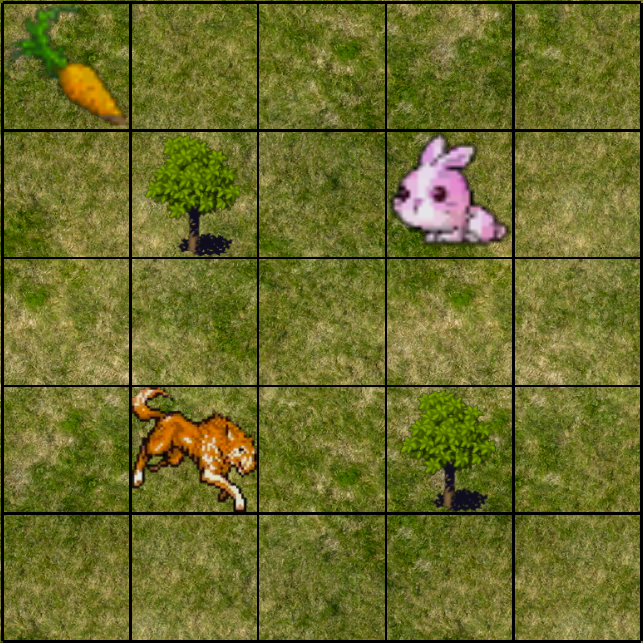
\includegraphics[height=2.4in]{bunny.png}
\end{center}


\caption{In the grid world above, the bunny must pursue two goals simultaneously: find food and avoid the wolf.  The bunny may move up, down, left, or right.  When it finds food it consumes the food and new food appears elsewhere in the grid world, when it meets the wolf it is eaten and ``respawns'' elsewhere.}
\label{fig:bunny-picture}
\end{figure}

In this task each programmer wrote an agents that control a bunny character in a simple world, depicted in Figure~\ref{fig:bunny-picture}.  The bunny world works as follows:

\begin{itemize}

\item The bunny world is a discrete grid of cells.  The bunny, wolf, and food each occupy one cell.

\item During each time step the bunny may move north, south, east, or west -- this is the bunny agent's action set.

\item Every two time steps the wolf moves towards the bunny.

\item If the bunny moves to the cell currently occupied by the food, the agent should be written to recognize this fact and give the agent an appropriate reward signal. In any case the simulation assumes food is ``eaten'' and new food appears elsewhere.

\item If the wolf moves to the cell currently occupied by the bunny it eats the bunny and the bunny ``respawns'' in a new location.

\end{itemize}

Programmers were asked to write bunny agents that meet the wolf as little as possible and eat as much food as possible.

\subsection{Task 2: Mating Bunny}\label{sec:task2}

In this task each programmer wrote a bunny agent for a world that is identical to the world in Task 1 except that the bunny must also find mates.  This world includes one static  potential mate that behaves similarly to the food.  When the bunny finds the potential mate, the simulation assumes that the bunny has ``mated,'' the mate disappears, and another potential mate appears elsewhere.  The simulation runs as in Task 1, and the scorer additionally keeps track of how many mates the bunny finds.  As in Task 1, programmers were asked to write bunny agents that meet the wolf as little as possible, eat as much food as possible, and find as many mates as possible.

\subsection{Provided Code}

Study participants were given starter code so they could focus on writing the behavior of their agents. We provided the world for each task and the files in which to write their code. Participants were also given general documentation for AFABL but assumed to already be proficient in Scala.

Figure \ref{fig:scala-task1-provided} shows the code given to participants for the Scala bunny on Task 1. Figure \ref{fig:afabl-task1-provided} shows the code given to participants for the AFABL bunny on Task 1. The {\tt BunnyWorld}, {\tt BunnyState}, and {\tt BunnyAction} classes were also provided. It was up to participants to write state abstraction classes if they chose to do so.


\begin{figure}[!h]
\begin{center}

\begin{lstlisting}[language=Scala]
class ScalaBunny1 extends Agent[BunnyState, BunnyAction.Value]
    with Task1Scorer {

  // Your code goes in the body of this method. This method defines
  // your agent's behavior, that is, what action it takes in a given
  // state. The last expression in this method must be a
  // BunnyAction.  You may create as many helper functions as you
  // like, but please do not alter any of the provided code.
  def getAction(state: BunnyState, shouldExplore: Boolean = false) = {

    // This is a stub to make the code compile. Please
    // replace this with your code.
    BunnyAction.Up
  }
}
\end{lstlisting}

\caption{Starter Scala code provided to participants for Task 1.}
\end{center}
\label{fig:scala-task1-provided}
\end{figure}


\begin{figure}[!h]
\begin{center}

\begin{lstlisting}[language=Scala]
object AfablTask1 {

  // Use this val in your agent definitions.
  val bunnyWorld = new BunnyWorld

  // Please place all of your AFABL code for Task 1 in this singleton
  // object.


  // Your solution must assign your AFABL bunny agent for Task 1 to
  // the val afablBuny1.
  val afablBunny1 = ???
}
\end{lstlisting}

\caption{Starter AFABL code provided to participants for Task 1.}
\end{center}
\label{fig:afabl-task1-provided}
\end{figure}


The provided code for Task 2 was identical to the provided code for Task 1, except for the names of the files. For Task 2 participants were encouraged to copy code from Task 1 if they found it helpful, or to use any objects defined for Task 1 that would be helpful, such as behavior modules. As we discuss below, reusing code was straightforward for the AFABL agents but not for the Scala agents. As in Task 1, it was up to participants to write state abstraction classes if they chose to do so, but they could reuse any state abstraction classes written for Task 1.

Each task had a main method which ran the agents in the world to evaluate their performance.

\section{Quantitative Results}

We analyzed the submissions of study participants to compare Scala agents to AFABL agents in terms of code size, time spent writing Scala versus AFABL agents, the complexity of Scala versus AFABL agent code, and the performance of the agents on the assigned tasks.

\subsection{Code Size}

The size of a code base is often correlated with the level of effort required to write or understand the code. We computed the number of lines of code for each agent, not including comments.

\subsection{Time}

Study participants used the IntelliJ IDEA IDE with a plug-in that we wrote especially for this study. The plug-in recorded timestamps each time the editor tab with Task 1 or Task 2 files gained or lost the focus. We processed these logs to add up the time deltas between gaining and losing focus as an indication of the time programmers spent writing the code for each bunny agent.

\subsection{Cyclomatic Complexity}

We computed a complexity measure for all the submitted bunny agents. For Scala code we employed the simplified McCabe cyclomatic complexity measure \cite{mccabe1976complexity}:

\begin{equation}
v = \pi + 1
\end{equation}

where $v$ is the complexity score and $\pi$ is the number of predicates in decision structures.

\subsection{Performance}

Each programmer's Scala bunny and AFABL bunny were run for 1000 time steps and their average scores recorded. The score is based on how much food the bunny eats and how many times the bunny is eaten by the wolf for Task 1, and additionally how many times the bunny mates for Task 2. The score is normalized by the number of steps to indicate a sort of ``happiness index,'' a ratio of rewards to lifespan. This score happens to correspond to the measure used to validate Arbi-Q in Chapter \ref{ch:arbiq} to facilitate comparison between programmer authored agents and the performance of the algorithms we implemented for our reformulated MRL. It is important to note, however, that our aim here is not to achieve optimal performance but to create a programming system that makes it easy to write agents that achieve good performance.

\subsection{Typical Task 1 Submissions}

\begin{figure}[!h]
\begin{center}

\begin{lstlisting}[language=Scala]
class ScalaBunny1 extends Agent[BunnyState, BunnyAction.Value]
    with Task1Scorer {

  def getAction(state: BunnyState, shouldExplore: Boolean = false) = {
    if (wolfNearFood(state))
      moveAwayFromWolf(state)
    else
      moveTowardFood(state)
   }

  def wolfNearFood(state: BunnyState) = {
    val wolfToFood = sqrt(pow(state.food.x - state.wolf.x, 2) +
                          pow(state.food.y - state.wolf.y, 2))
    val bunnyToFood = sqrt(pow(state.food.x - state.bunny.x, 2) +
                           pow(state.food.y - state.bunny.y, 2))
    wolfToFood < bunnyToFood
  }

  def moveTowardFood(state: BunnyState) = {
    if (state.food.x > state.bunny.x)
      BunnyAction.Right
    else if (state.food.x < state.bunny.x)
      BunnyAction.Left
    else if (state.food.y < state.bunny.y)
      BunnyAction.Up
    else
      BunnyAction.Down
  }

  def moveAwayFromWolf(state: BunnyState) = {
    if (state.wolf.x < state.bunny.x)
      BunnyAction.Right
    else if (state.wolf.x > state.bunny.x)
      BunnyAction.Left
    else if (state.wolf.y > state.bunny.y)
      BunnyAction.Up
    else
      BunnyAction.Down
  }
}
\end{lstlisting}

\caption{Typical Scala submission for Task 1.}
\end{center}
\label{fig:scala-task1-submission}
\end{figure}

Figure \ref{fig:scala-task1-submission} shows a typical Scala submission for Task 1. The action selection strategy is about as simple as possible. For example, there is no determination of where the wolf is in relation to the bunny and food other than distance. If the wolf is closer to the food than the bunny, move away from the wolf, otherwise move toward to the food. The agent does not distinguish between cases where the wolf is between the wolf and the food, or if the wolf is closer but sufficiently far away. One could imagine writing code to calculate the projection of the wolf's position onto the line between the bunny and the food to determine a safe closure rate for the wolf. However, this simple strategy is all that is needed to achieve nearly optimal results. This Scala-only bunny agent achieves an average performance score of 0.54, the same as the AFABL bunny.

\begin{figure}[!h]
\begin{center}

\begin{lstlisting}[language=Scala]
  case class FindFoodState(bunny: Location, food: Location)
  val findFood = AfablModule(
    world = bunnyWorld,
    stateAbstraction = (worldState: BunnyState) => {
      FindFoodState(worldState.bunny, worldState.food)
    },
    moduleReward = (moduleState: FindFoodState) => {
      if (moduleState.bunny == moduleState.food) 1.0
      else -0.1
    }
  )

  case class AvoidWolfState(bunny: Location, wolf: Location)
  val avoidWolf = AfablModule(
    world = bunnyWorld,
    stateAbstraction = (worldState: BunnyState) => {
      AvoidWolfState(worldState.bunny, worldState.wolf)
    },
    moduleReward = (moduleState: AvoidWolfState) => {
      if (moduleState.bunny == moduleState.wolf) -0.1
      else 0.1
    }
  )

  val afablBunny1 = AfablAgent(

    world = bunnyWorld,

    modules = Seq(findFood, avoidWolf),

    agentLevelReward = (state: BunnyState) => {
      if (state.bunny == state.wolf) 0.0
      else if (state.bunny == state.food) 1.0
      else 0.5
    }
  )
\end{lstlisting}

\caption{Typical AFABL submission for Task 1.}
\end{center}
\label{fig:afabl-task1-submission}
\end{figure}

Figure \ref{fig:afabl-task1-submission} shows a typical AFABL submission for Task 1. As in our earlier examples, the AFABL bunny is composed of behavior modules for finding food and avoiding the wolf. The AFABL documentation contained tips for reward authoring in modules and at the agent level.


The AFABL solution to Task 1 contains 31 lines of code and has a cyclomatic complexity of 5 (4 predicates in decision structures). The Scala solution to Task 1 uses 34 lines of code and has a cyclomatic complexity of 8 (7 predicates in decision structures). Both programs achieve the same nearly optimal level of performance with scores of ~0.54.

\subsection{Typical Task 2 Submissions}

\begin{figure}[!h]
\begin{center}

\begin{lstlisting}[language=Scala]
class ScalaBunny2 extends Agent[BunnyState, BunnyAction.Value]
    with Task2Scorer {

  def getAction(state: BunnyState, shouldExplore: Boolean = false) = {

    if ((distance(state.wolf, state.food) < distance(state.food, state.bunny))
      || distance(state.wolf, state.mate) < distance(state.mate, state.bunny))
      moveAwayFromWolf(state)
    else if (distance(state.bunny, state.food) < distance(state.bunny, state.mate))
      moveToward(state.bunny, state.food)
    else
      moveToward(state.bunny, state.mate)
  }

  def distance(a: Location, b: Location) = {
    sqrt(pow(a.x - b.x, 2) + pow(a.y - b.y, 2))
  }

  def moveToward(from: Location, to: Location) = {
    if (to.x > from.x)
      BunnyAction.Right
    else if (to.x < from.x)
      BunnyAction.Left
    else if (to.y > from.y)
      BunnyAction.Up
    else
      BunnyAction.Down
  }

  def moveAwayFromWolf(state: BunnyState) = {
    if (state.wolf.x < state.bunny.x)
      BunnyAction.Right
    else if (state.wolf.x > state.bunny.x)
      BunnyAction.Left
    else if (state.wolf.y > state.bunny.y)
      BunnyAction.Up
    else
      BunnyAction.Down
  }
}
\end{lstlisting}

\caption{Typical Scala submission for Task 2.}
\end{center}
\label{fig:scala-task2-submission}
\end{figure}

Figure \ref{fig:scala-task2-submission} shows a typical Scala solution for Task 2. While the Scala solution to Task 2 is more complex than the Scala solution to Task 1, it uses only one more line of code -- 35 -- due to refactoring of common logic. Of course, this refactoring took extra time and without the refactoring the line count and likely the cyclomatic complexity would have been higher.

\begin{figure}[!h]
\begin{center}

\begin{lstlisting}[language=Scala]
  case class FindMateState(bunny: Location, mate: Location)
  val findMate = AfablModule(
    world = bunnyWorld,
    stateAbstraction = (state: BunnyState) => {
      FindMateState(state.bunny, state.mate)
    },
    moduleReward = (state: FindMateState) => {
      if (state.bunny == state.mate) 1.0
      else -0.1
    }
  )

  // Your solution must assign your AFABL bunny agent for Task 2 to
  // the val afablBuny2.
  val afablBunny2 = AfablAgent(

    world = bunnyWorld,

    modules = Seq(AfablTask1.findFood, AfablTask1.avoidWolf, findMate),

    agentLevelReward = (state: BunnyState) => {
      if (state.bunny == state.wolf) 0.0
      else if (state.bunny == state.food) 1.0
      else if (state.bunny == state.mate) 1.0
      else 0.5
    }
  )
\end{lstlisting}

\caption{Typical AFABL submission for Task 2.}
\end{center}
\label{fig:afabl-task2-submission}
\end{figure}

Figure \ref{fig:afabl-task2-submission} shows typical AFABL code for Task 2. Notice that the {\tt findFood} and {\tt avoidWolf} modules from Task 1 have been reused directly. This works because the world, {\tt BunnyWorld}, is the same. In Task 1 the bunny was ignoring the mate. In Task 2 we adapt the bunny to find the mate, and all we need to do is add a {\tt findMate} module and add a line to the {\tt agentLevelReward} function so that the agent will also value finding mates.

The AFABL solution to Task 2 contains 21 lines of code due to reuse of modules from Task 1, and has the same cyclomatic complexity of 5 (4 predicates in decision structures) even though the agent is solving a more complex problem. Even with the refactoring of common logic in Task 2 the Scala solution has a higher cyclomatic complexity of 10 (9 predicates in decision structures), which McCabe says is the maximum allowable cyclomatic complexity for a testable, maintainable software module \cite{mccabe1976complexity}. Finally, the performance of the Scala solution to Task 2 decreases to 0.48, while the AFABL solution continues to achieve the same nearly optimal 0.54. With additional work perhaps the Scala agent's performance on Task 2 could have been improved, but the point here is that AFABL agents are easier to write, easier to adapt to new domains, have less complex code, and perform well without requiring a great deal of effort beyond choosing reward signals.

\subsection{Summary}

Quantitative results for Task 1 are summarized in Table \ref{tbl:task1-results}. Quantitative results for Task 2 are summarized in Table \ref{tbl:task2-results}.

\begin{center}
\begin{table}[h]
\begin{tabular}{|l|r|r|r|}\hline
                      & Scala Mean & AFABL Mean & p-value \\\hline
Lines of Code         & 0.0        & 0.0        & 0.0 \\
Time                  & 0.0        & 0.0        & 0.0 \\
Cyclomatic complexity & 0.0        & 0.0        & 0.0 \\
Performance           & 0.0        & 0.0        & 0.0 \\\hline
\end{tabular}
\caption{Quantitative results of Scala agent code versus AFABL agent code on Task 1. A p-value of less than .05 mean that the difference in means is statistically significant at the 95\% significance level, i.e. we reject $H_0: \mu_1 = \mu_2$ and conclude that the means are different.}
\label{tbl:task1-results}
\end{table}
\end{center}

\begin{center}
\begin{table}[h]
\begin{tabular}{|l|r|r|r|}\hline
                      & Scala Mean & AFABL Mean & p-value \\\hline
Lines of Code         & 0.0        & 0.0        & 0.0 \\
Time                  & 0.0        & 0.0        & 0.0 \\
Cyclomatic complexity & 0.0        & 0.0        & 0.0 \\
Performance           & 0.0        & 0.0        & 0.0 \\\hline
\end{tabular}
\caption{Quantitative results of Scala agent code versus AFABL agent code on Task 2. A p-value of less than .05 mean that the difference in means is statistically significant at the 95\% significance level, i.e., we reject $H_0: \mu_1 = \mu_2$ and conclude that the means are different.}
\label{tbl:task2-results}
\end{table}
\end{center}

\section{Qualitative Results}

Programmers responded to a questionnaire to give their impressions of agent programming in AFABL versus agent programming in Scala.

\begin{enumerate}
\item I have a positive impression of agent programming in Scala.

Rationale: programmers’ impression of Scala will provide a baseline for evaluating
programmers’ impression of AFABL.

\item I found it easier to write the agents using AFABL’s programming constructs compared to bare Scala.

Rationale: the point of AFABL is to facilitate agent programming, so programmers should have a more positive impression of AFABL for agent programming.

\item I believe that AFABL facilitated more reusable and maintainable code for agents compared to bare Scala.

Rationale: answers to this question should correlate with answers to Question 1.

\item If given the choice, I would choose AFABL over Scala for agent programming projects.

Rationale: answers to this question should correlate with answers to Question 2.

\item I found it easier to use AFABL compared to Scala for Task 1.

  Rationale: in addition to objective analyses of task submissions, we want to know whether programmers subjectively prefer AFABL.

\item What was it about AFABL that made the Task 1 easier or harder?

Rationale: we want to get open-ended feedback for things we did not anticipate.

\item I found it easier to use AFABL compared to Scala for Task 2.

Rationale: in addition to objective analyses of task submissions, we want to know whether programmers subjectively prefer AFABL.

\item What was it about AFABL that made the Task 2 easier or harder?

\end{enumerate}

\section{Threats to Validity}

Sample size

Problem size

TAs as subjects

\section{Conclusion}

As you can see from the similarity of the submission in Figure \ref{fig:afabl-task1-submission} to our explanatory example, most AFABL bunny agents look the same. There is one obvious way to implement a bunny agent that must pursue multiple goals. This uniformity is desirable. As Tim Peters says in the Zen of Python \cite{peters2004zen}, ``There should be one-- and preferably only one --obvious way to do it.'' The similarity in most AFABL solutions to a particular modular agent programming problem is an indication that AFABL provides the right abstractions for adaptive agent programming.
